\documentclass[10pt, titlepage]{report}

\usepackage[utf8]{inputenc}
\usepackage[T1]{fontenc}
\usepackage[francais]{babel}

%Caractères spéciaux

\usepackage{lmodern}
\usepackage{amsmath}
\usepackage{amssymb}
\usepackage{mathrsfs}

\usepackage{eurosym} %insertion signe euro
\usepackage{graphicx} %insertion d'images
\usepackage{fancyhdr} %en-tete et pied de page

\title{\bsc{Rapport de la deuxième soutenance}\\Projet flight arena}
\author{mr cube :\\
Vincent \bsc{Rospini-Clerici},\\
Guillaume \bsc{Rebut}\\
%Nikolas \bsc{Miletic}\\
chef de projet : Arthur \bsc{Remaud}}
\date{7 mai 2015}

\pagestyle{fancy}
\fancyhead{}
\fancyfoot{}
\lhead{Rapport de la deuxième soutenance}
\rhead{Projet flight arena}
\lfoot{mr cube}

\begin{document}

\maketitle
\renewcommand{\contentsname}{Sommaire}
\renewcommand{\chaptername}{Partie}

\tableofcontents

\begin{center}
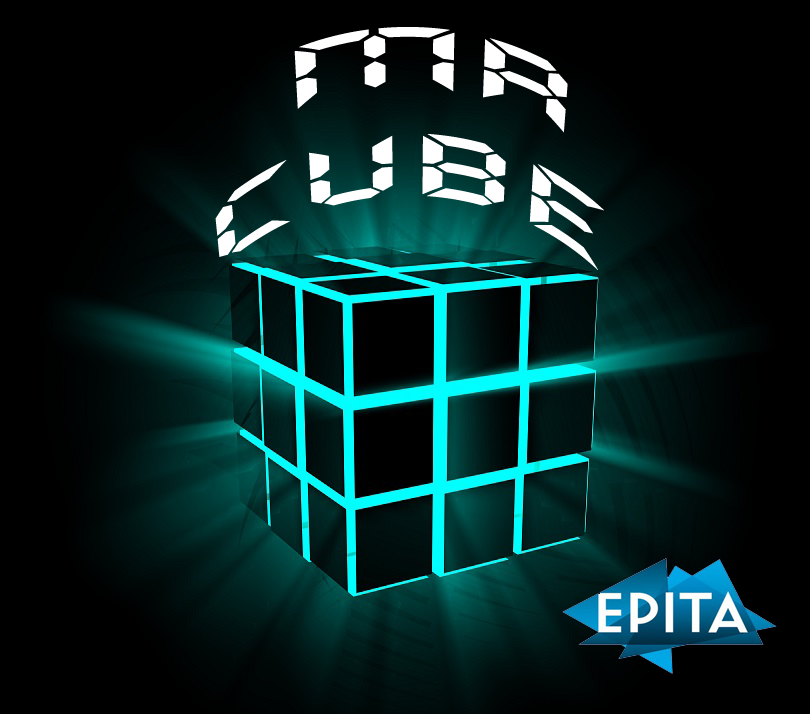
\includegraphics[height=8cm, width=9cm]{MRCUBE.PNG}
\end{center}

\chapter{Rappel de la première soutenance}
A la première soutenance, nous avions présenté une première carte avec d’ores et déjà des bâtiments en trois dimensions. Il y avait plusieurs vaisseaux faits avec Blender pour la modélisation et Photoshop pour les textures, mais un seul était réellement assez beau et vraiment fini.\\

\begin{center}
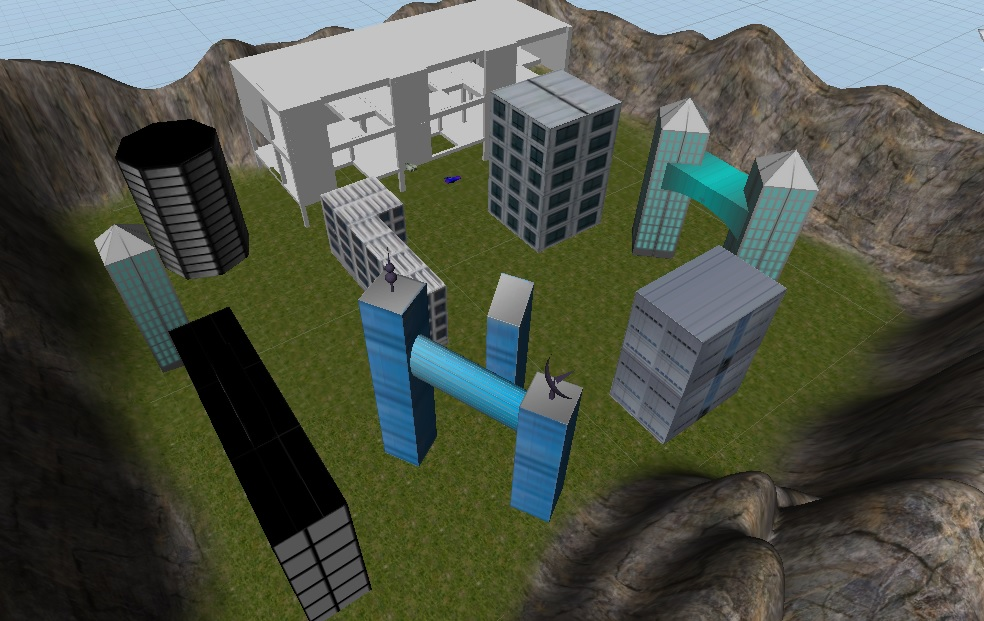
\includegraphics[height=6cm, width=10cm]{carte.jpg}
\end{center}

Il y avait les déplacements et les tirs du joueur intégrés aux contrôles en utilisant les fonctions \textit{Rotate}, \textit{Translate} et \textit{Instanciate}. Nous avions donc déjà les bases du gameplay et la physique était bien avancée : les collisions étaient déjà intégrées et le terrain était délimité. La vie du vaisseau n’était pas encore implémentée dans le jeu.La pause avait été aussi insérée dans le jeu, que ce soit pour aller dans les options, pour revenir au menu ou pour quitter le jeu. \\

Le menu contenait déjà les principaux onglets : jouer, multijoueur, options, quitter. La musique du menu avait été choisie pour être celle du thème de \textit{Captain America}. Cependant, certains boutons n'aboutissaient sur rien car le contenu n'avait pas été fait (le multijoueur surtout), mais le menu option avait été entamé avec la gestion du volume de la musique et des bruitages qui était conservé en mémoire même après avoir fermé le jeu grâce à la classe \textit{PlayerPrefs}.\\

Il nous avait été signalé que les déplacements du vaisseau seraient mieux si nous utilisions des quaternions pour les rotations, pour avoir un rendu plus réaliste. Ces derniers créant des problèmes avec les collisions du vaisseau, raison pour laquelle nous ne les avions pas utilisés, c'était donc un de nos principaux défis pour la seconde soutenance.\\
Nous partions donc sur de bonnes bases lors de la première soutenance, car nous avions d’ores et déjà un jeu jouable et amusant qui nous permettait de se déplacer et de tirer avec un vaisseau sur toute la carte. \\

\chapter{Retard/Avance par rapport au cahier des charges}

\section{Prévisions}
A l'issue de la première soutenance nous avions prévu pour la seconde soutenance d'améliorer le contenu du jeu en ajoutant de nouvelles modélisations et des paramètres dynamiques, de créer une intelligence artificielle qui fonctionne correctement, et un site web quasiment opérationnel.\\

 Le multijoueur en écran scindé, en LAN, ou en réseau devait aussi être ébauché. Le menu des options devait être complété, et il fallait rajouter la sélection du vaisseau au démarrage de la partie.\\

Le site internet devait être commencé et contenir les informations de base autour du projet.\\

A la suite d'une remarque lors de la première soutenance, nous devions aussi refaire les déplacements avec des quaternions pour les rendre plus réalistes avec les effets d'inertie.\\

\section{Retard}

\subsection{Intelligence artificielle}
En voulant d'ores et déjà nous concentrer sur le multijoueur, nous avons reporté la finalisation de l'intelligence artificielle à plus tard. L'intelligence artificielle qui est actuellement sur le jeu fonctionne en essayant d'éviter les obstacles mais ne cherche pas à détruire le vaisseau adverse.\\

\subsection{Cartes}
Nous n'avons pas eu le temps d'élaborer de nouvelles cartes pour jouer sur un terrain différent. Nous avons préféré mettre l'accent sur le multijoueur et les ajouts de fonctions comme l'affichage de la vie et une horloge sur l'écran.\\

\subsection{Option changer de touches de commande}

Nous voulions rajouter dans le menu des options la possibilité de choisir ses propres touches sur le clavier pour piloter le vaisseau et faire en sorte que le jeu le retienne. Cependant, nous ignorons totalement comment le faire et aucun site internet ne parle de cela.

Comme Unity, de base, permet au démarrage d'assigner ses touches, et que cela n'est qu'un bonus pas nécessaire, nous avons donc abandonné notre idée de base.\\

\section{Avance}

\subsection{Multijoueur}
Le multijoueur était dans les prévisions la priorité entre la seconde soutenance et la soutenance finale. Mais, nous nous sommes finalement ravisé d'attendre pour le commencer, car notre projet, venant tout d'abord de l'idée de créer un jeu en arène pour que les joueurs puissent s'affronter entre eux. Or, la création d'intelligence artificielle en amont aurait considérablement ralenti l'arrivée d'un multijoueur jouable. Désormais, le jeu est jouable, que ce soit en écran scindé ou en LAN.\\

Finalement, l'avance prise sur le multijoueur compense le retard pris dans l'intelligence artificielle : nous avons juste inversé les prévisions entre la deuxième et la dernière soutenance.

\chapter{Travail par membre}
Nous allons vous décrire ce que chaque membre de l'équipe mr cube a fait pendant cette deuxième période, avec leurs difficultés rencontrées et les techniques utilisées.

\section{Guillaume Rebut}

\subsection{Écran Partagée} 
 Parce que de moins en moins de jeu proposent un écran partagé (alors que les écrans s'agrandissent de plus en plus) et que le nombre de jeux de tirs multijoueur sur un seul clavier se comptent sur les doigts de la mains, nous avons décidé de créer un multijoueur en écran scindé.
Le joueur 1 utilisera les touches (pour un clavier qwerty) A/D pour le lacet, H/K pour le roulis et U/J pour le tangage. Le joueur 2 utilise les touches flèche de droite/flèche de gauche pour le lacet, 4/6 (du pave numérique) pour le roulis et touche flèche du haut/flèche du bas pour le tangage. \\

\begin{center}
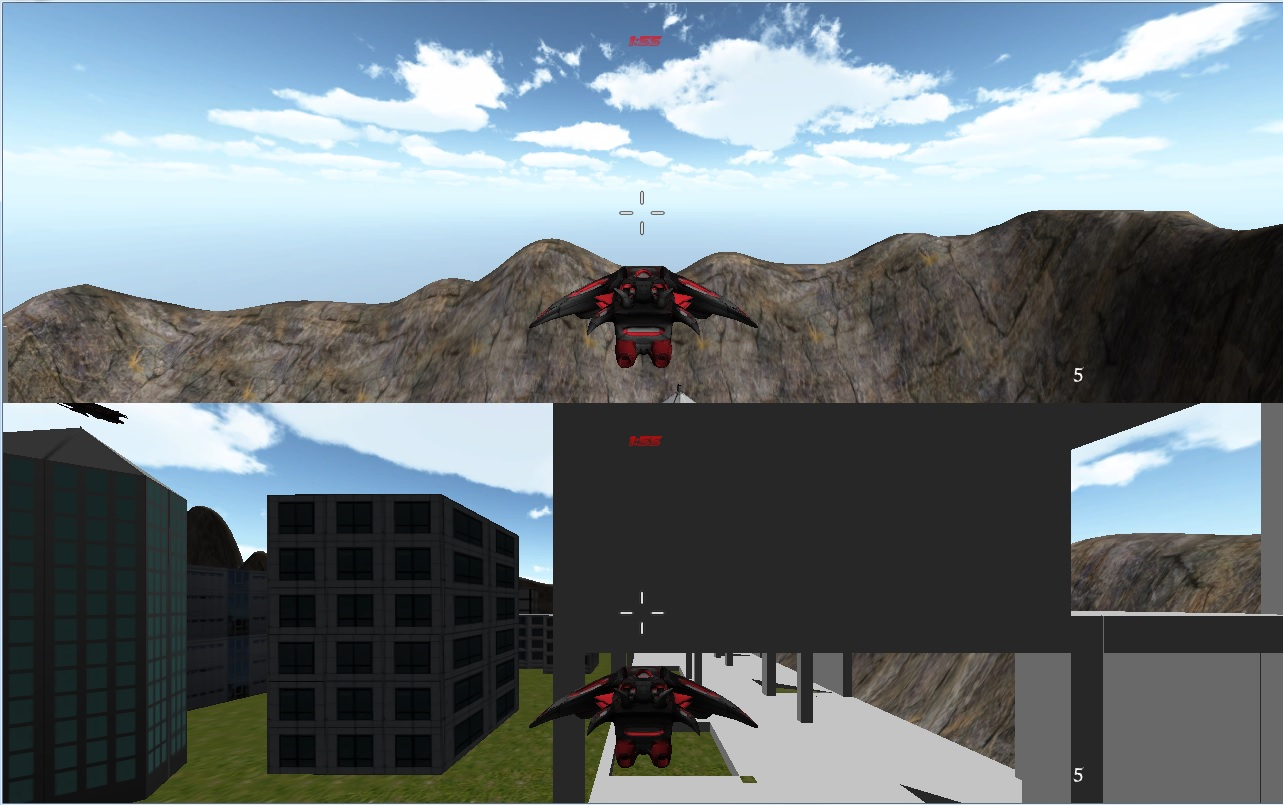
\includegraphics[height=5cm, width=9cm]{split.jpg}
\end{center}

\subsection{Premier mode de jeu} Le premier mode de jeu est un match à mort chacun pour soi. Le joueur gagne quand un vaisseau ennemi explose ou s'il a le plus de points de vie après la fin du temps imparti.\\
 
\subsection{Son} 
 Nous avons ajouté un court bruit qui se joue lorsque un joueur touche un vaisseau ennemi, pour aider le joueur. En effet, cela permet au joueur de déduire les points de vies restants de son adversaire et de réagir en fonction.\\

\subsection{Mouvement}
Suite aux recommandations des évaluateurs, nous avons décidés de rendre le contrôle du vaisseau moins "arcade". Pour cela, en plus de l'ajout de quaternion, nous avons souhaités rendre les déplacements du vaisseau réaliste. En effet, lorsque l'utilisateur ne fait pas avancer le vaisseau, ce dernier s'immobilise rapidement dans les airs. Pour résoudre ce problème, nous avons décidé d'implémenter les vrais équations de mouvements des avions.\\

 L'équation qui nous intéresse le plus est la suivante : R = 1/2 Cx  p S v.v . Soit la résistance de l'air est égale a la moitie de la surface du vaisseau fois la constante de trainée fois la masse volumique de l'air fois la vitesse au carré, ce que nous avons simplifié par la vitesse au carre fois une constante. Lors des premiers essais, la vitesse était calculée en soustrayant la force de frottement a l'accélération. Cette méthode donnait des résultats satisfaisant car les mouvements était fluide et le vaisseau ne s'arrêtait jamais. Cependant, pour une raison indéterminée, si le joueur décidait de ne pas avancer après avoir réapparu, le vaisseau avait une vitesse négative qui devenait très importante très rapidement et sortait le vaisseau des limites de unity.\\

Le problème disparu lorsque nous utilisions \textit{Transform.translate} qui prend en paramètre un vector 3. Nous avons ensuite implémentés une option permettant au joueur de freiner. Cette option retrancher une valeur fixe a la vitesse tant que celle ci était positive. Cependant, malgré toute les précautions prises, notre problème de vitesse négative est réapparus . La solution prise fut d'augmenter la valeur de la force de frottement.\\

La prochaine étape fut d'implémenter la portance. Ceci signifie aussi qu'il fallait implémenter la gravité. Nous avons du pour cela passer d'une modification de la vitesse grâce a \textit{Transform.translate} a une modification de la vélocité du \textit{rigidbody} du vaisseau. Cependant, l'implémentation de la portance implique une force relative au monde et non au vaisseau. Cette étape ne fut pas d'une grande difficulté mais l'ordre de grandeur des valeurs est différente que celle du référentielle vaisseau. Ce détail nous a empêché de trouve la valeur exacte de manière a ce qui le vaisseau vole en ligne droite lorsqu'il est parallèle au sol, ce qui veut dire que le joueur est tout le temps oblige de compenser cette force, ce qui devient vite ennuyant. Nous avons finalement décider d'enlever les frottements ainsi que la possibilité de freiner.\\

\subsection{Interface Graphique  Utilisateur}

\subsubsection{Cibleur}
 Pour des raisons de gameplay, les missiles du vaisseau ne se dirigent pas tous vers le même point mais recouvrent un petite zone. Nous affichons donc, pour aider le joueur, cette zone sur l'écran. Cette zone est délimitée par quatre rectangles blancs. Pour faciliter les manipulations, ces quatre rectangles ont des coordonnées pour que tous bougent quand l'un bouge. \\

\begin{center}
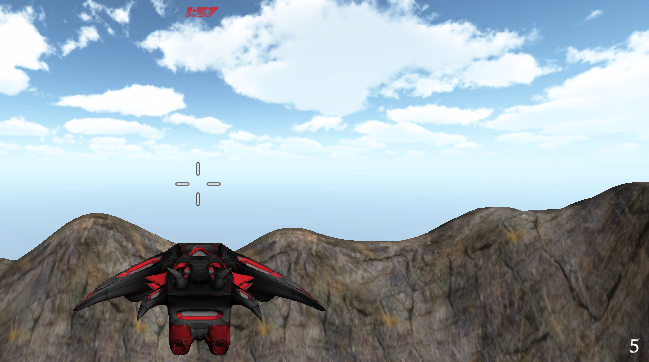
\includegraphics[height=6cm, width=9cm]{Capture_rebut.PNG}
\end{center}

\subsubsection{Horloge}
Nous avons implémentes un une horloge qui limite le temps de jeu. Lorsque que le temps imparti est dépassé, la partie s'arrête, et le vainqueur est détermine de la manière suivante : un frag vaut 1 point, une mort -0.5 point et le joueur gagnant est affiche a l'écran. En cas d'égalité, le jeu indique que les joueurs ont fait match nul.\\

\subsection{Réapparition des vaisseaux}  
Faire réapparaitre les vaisseaux sur des points prédéfinis présente un grand avantage car le vaisseau ne sera jamais dans un mur ou en dehors des limites de la carte. Cependant cela veut dire que le joueur est capable de créer des boucles de réapparitions de manière a tuer son adversaire des qu'il réapparait.Nous avons donc choisis de faire réapparaitre les vaisseaux aléatoirement en gérant les cas ou ils seraient en dehors des limites et les cas ou ils réapparaissent dans un objet.\\

De plus, pour vraiment donner l'impression que le vaisseau a disparu, le script désactive l'émetteur de particule produisant les flammes du vaisseaux. Nous immobilisons aussi le vaisseau. Pour cela, le script désactivait d'abord le \textit{gameobject} du vaisseau. Cette solution qui semble facile présente en réalité beaucoup de désavantages : les valeurs de mouvements et de rotations sont conservées ce qui veut dire que le vaisseau ne réapparait pas en étant immobile. De plus, nous avons ajouté le script de réapparition au vaisseau, ce qui veut dire que désactiver le \textit{gameobject} vaisseau désactive aussi le script de réapparition.\\

 La solution que nous avons choisi est la suivante : nous immobilisons dans un premier temps le vaisseau en réinitialisant ses valeurs de rotations et de vitesses. Le script  rend ensuite le vaisseau invisible en désactivant les \textit{mesh rendert} de ses différents composants et en désactivant les collisions. Après un (très) court temps d'attente, le vaisseau réapparait sur une autre position et retrouve une valeur de points de vie prédéfinie.\\

\subsection{Portage du jeu}

Le jeu fut d'abord développé pour la partie écran scindé, ce qui veut dire que les scripts fonctionnaient par exemple en supposant que l'on sait d'avance combien de vaisseaux sont présents, qu'ils ont tous le même émetteur de particules  ou le même nombre de \textit{mesh}. Lors de la création de la partie multijoueur, il devint nécessaire que les scripts puissent fonctionner sans ces contraintes. Le défi fut que chaque fonctions tiennent sur le même script respectif, donc que l'on n'ait pas à créer un script par vaisseau.\\


\subsection{Ce que Guillaume doit faire pour la soutenance finale}

Le plus important est de finir la deuxième carte en cours de développement. Cette carte sera plus grande que la première pour permettre une meilleur visibilité mais aussi pour permettre de plus grandes manœuvres. Une troisième carte sera aussi finie et servira de  carte d'entrainement pour les débutants : ils seront d'abord initiés au différents mouvements du vaisseau, passeront des exercices leur demandant de slalomer entre des obstacles, s'entraineront a tirer sur des cibles immobiles puis mouvantes. Cette carte proposera aussi de jouer contre une intelligence artificielle.\\

Le jeu proposera plusieurs modes de jeu : celui en développement, un match a mort par équipe, ainsi que d'autres modes de jeu se basant sur des objectifs (par exemple capture du drapeau, contrôle de territoire, roi de la colline, infection,etc).\\

Le jeu proposera aussi plus d'options de jeu une interface graphique utilisateurs plus poussée et une intelligence artificielle amélioré.\\

\section{Vincent Rospini-Clerici}

\subsection{Création de nouveaux vaisseaux}
Dans le soucis d'ajouter du contenu, deux nouveaux vaisseaux ont été créés sur Blender et textures sur Photoshop. Il s'agit tout d'abord d'un vaisseau qui ferait penser à un jet militaire tout droit venu du futur. L'autre est inspiré du P40, un avion militaire américain utilisé durant la seconde guerre mondiale et auquel Vincent a rajouté des nacelles de missiles et des réacteurs pour lui donner un air à la fois futuriste et ancien. Deux textures ont été crées pour ce dernier vaisseau mais nous nous servirons pour le moment d'une seule d'entre elle pour la première soutenance.\\

\begin{center}
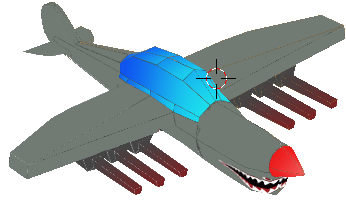
\includegraphics[height=3cm, width=5cm]{sharknado.png}
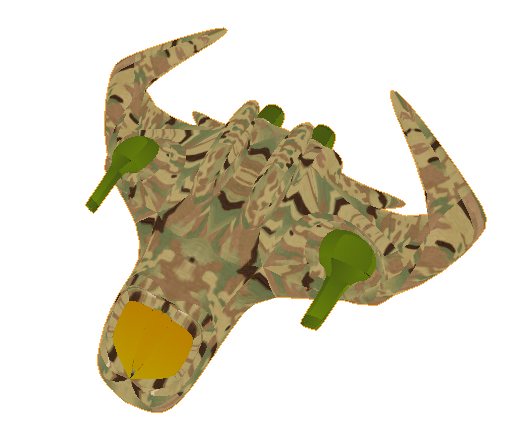
\includegraphics[height=3.5cm, width=5.5cm]{vaisseaumilitaire.png}
\end{center}


\subsection{Ajout des particules des vaisseaux}
Les flammes sortant des réacteurs des vaisseaux ont été rajoutes par le biais de la création de particules qu'offre Unity. Tout d'abord, Vincent a rajouté des éléments de particules pour créer juste des flammes sortant des réacteurs, mais le groupe s'est mis d'accord pour que les réacteurs laissent une trainée après le passage du vaisseau. Cependant, les particules étant contenu dans le \textit{gameobject} du vaisseau, les flammes tournaient lorsque le vaisseau tournait, au lieu de simplement suivre sa trajectoire. Nous avons après quelques recherches sur internet nous avons trouve le paramètre permettant de le faire. Il s'agissait de définir l'espace de simulation au niveau monde et non au niveau de l'objet.\\

\begin{center}
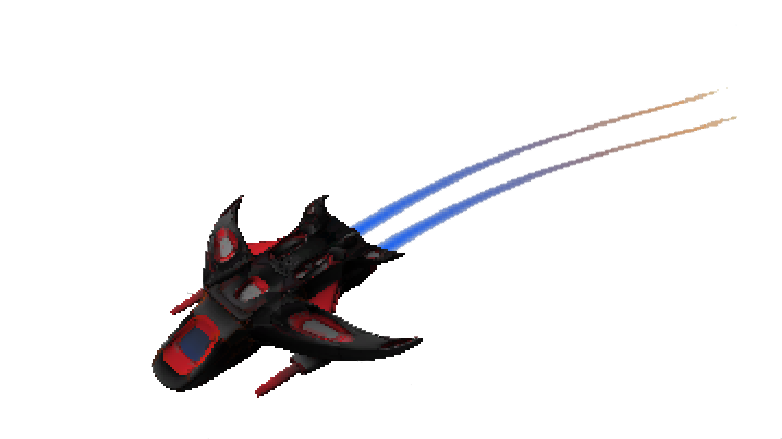
\includegraphics[height=3cm, width=5cm]{vaisseau_bouge.png}
\end{center}

Les trainées laissées par le réacteur sont différentes selon le vaisseau. Par exemple, l'avion laisse une trainée noire de fumée tandis que le vaisseau rouge et noir laisse une trainée bleu rectiligne. De cette façon, les vaisseaux adverses sont plus faciles à reconnaitre parmi les différents éléments de la carte. La création des particules pour la destruction du vaisseau a été commencée sur Unity. Elle se composera de plusieurs particules pour la fumée, les débris et les étincelles. Cependant, n'étant pas terminée, nous ne pouvons pas encore la dévoiler.  \\

\subsection{Création du site internet}
Vincent s'est occupé de la création du site internet en vue de la seconde soutenance. Il a décidé de créer le site en langage \textit{HTML} par le biais des logiciels d'adobe, Photoshop et DreamWeaver. Ce dernier est un logiciel permettant d'à la fois modifier directement le code du site et de s'occuper de son coté graphique plus aisément.\\

Il a voulu créer un site avec un design sombre qui rappellerait un ciel étoilé avec de nombreuses images des vaisseaux crées afin de le rendre attirant. Les pages du site ont été désignées sur Photoshop avec des images crées spécialement pour le fond d'écran et pour embellir les pages du site. Le site est prévu pour avoir toutes ses pages traduites en anglais et en français en cliquant simplement sur le drapeau correspondant a la langue voulue. Le site contiendra une page d'accueil,une page pour présenter le jeu, une pour présenter l'équipe et une pour que les visiteurs puissent avoir accès au cahier des charges, à l'exécutable du jeu, et peut-être à d'autres contenus à venir.\\

\begin{center}
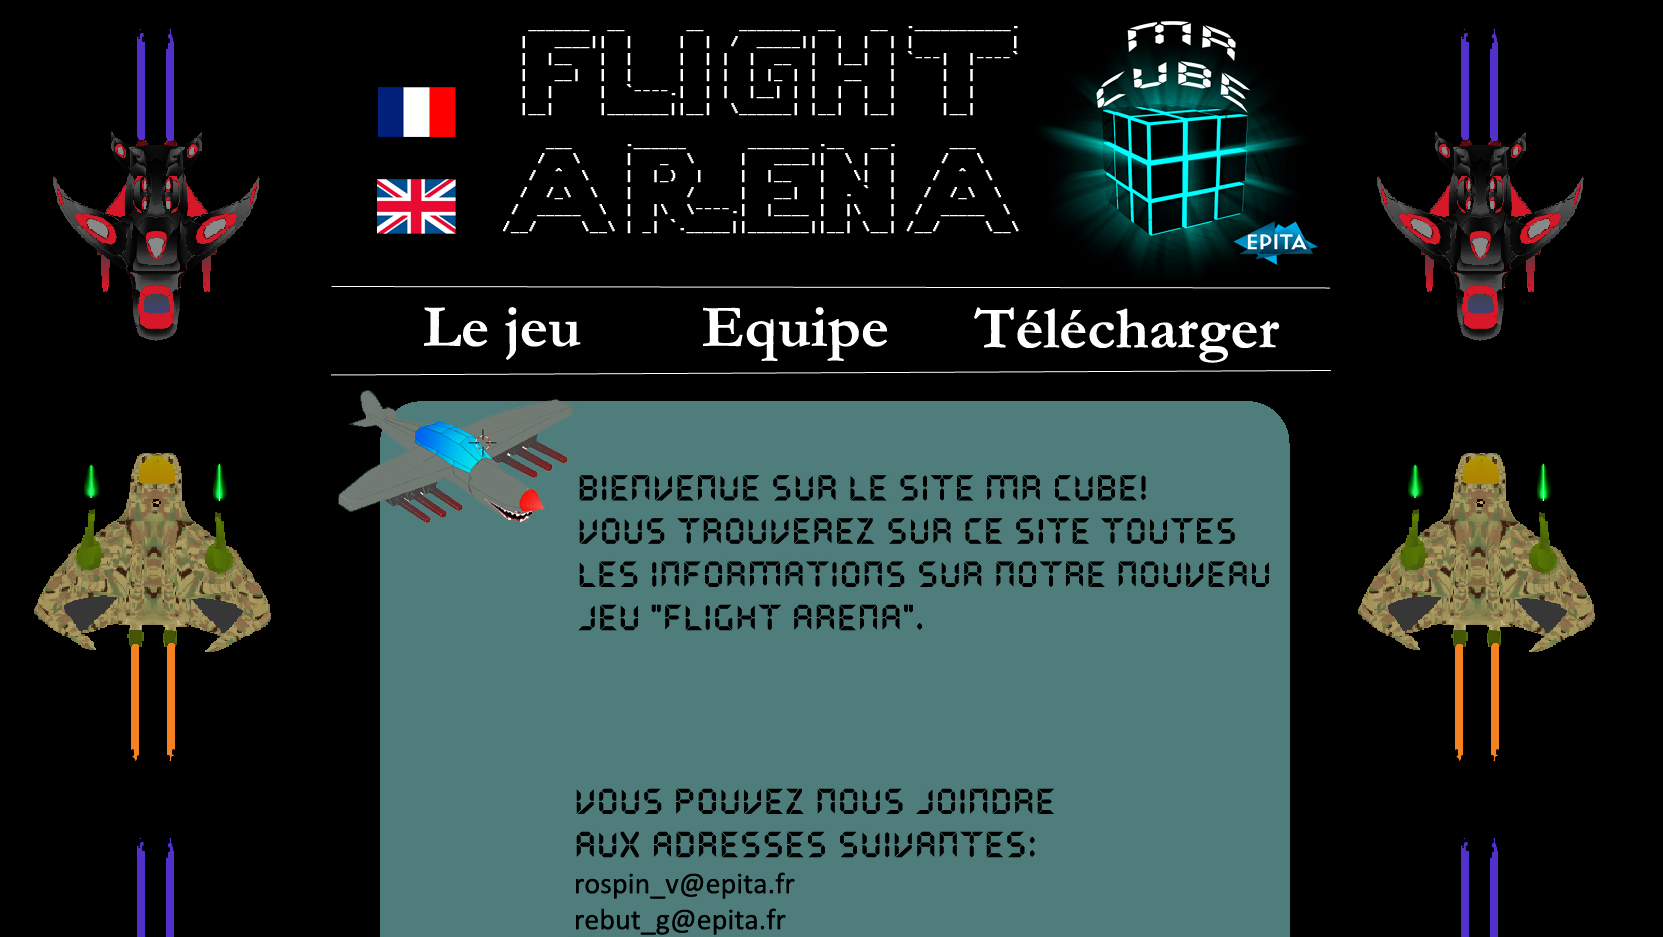
\includegraphics[height=6cm, width=10cm]{site.png}\\
aperçu du site internet
\end{center}

\subsection{Création d'une musique originale}
Nous avons finalement eu le temps et la patience de créer une \textit{original soundtrack} pour le jeu. Vincent a contacté un ami à lui qui fait des études musicales afin de savoir s'il était possible de créer des musiques en coopération avec lui. La réponse étant positive, deux musiques ont été créés à ce jour par notre ami assisté par Vincent par le biais du logiciel Logic Pro. \\

Nous souhaitions des musiques électroniques qui semblent futuristes, mais lentes. De ce fait, l'ambiance est angoissante et la peur de voir un ennemi surgir de derrière un bâtiment de la carte ou de se faire surprendre par derrière est présente.\\

"There's something beyond", une des deux musiques, a été ajoutée sur Unity et est écoutable dès lors qu'un joueur entre dans la partie. L'autre musique "Vincighilan" sera probablement ajoutée avec l'apparition d'une nouvelle carte ou d'un tutoriel.

\subsection{Ce que Vincent doit faire pour la soutenance finale}
Pour la soutenance finale, le site sera terminé et mis en ligne sur un serveur. La présentation du jeu sera ajoutée sur une nouvelle page du site pour les gens qui le découvrent. Cela permettra aux fans du jeu de se tenir au courant des dernières mises à jour. \\

Des nouveaux éléments de décor seront également créés sur la prochaine carte prévue pour le jeu. Nous avons actuellement une idée d’une carte avec des éoliennes dont les hélices tourneraient. Nous tenterons également d’ajouter de simples véhicules circulant et servant uniquement de décor. Les éoliennes et les véhicules seront modélisés et animées dans Blender évidemment. Créer de tels décors donnerait un coté très amusant à la carte, et c’est là une de nos priorité. \\

La destruction du vaisseau qui a déjà été commencée devra être rajoutée dans Unity. Elle est une part très importante du jeu. En sachant que nous n'arrivons pas à implanter la destruction du vaisseau de Blender dans Unity, nous allons donc faire disparaitre le vaisseau quand celui-ci sera détruit et rajouter des particules d'explosion et de débris pour masquer cette disparition soudaine. De ce fait, cette destruction sera réaliste.\\

L'apparition de nouveaux sons sera également a faire pour la soutenance finale. Nous choisirons différents sons pour étoffer le gameplay du jeu. Parmi ces différents sons a rajouter on compte le son d'une explosion qui sera rajoutée en même temps que la destruction du vaisseau, également un son lorsque le vaisseau entre en collision avec des éléments du décor, le bruit des réacteurs et peut-être d'autres selon l'avancée du projet.\\

\section{Arthur Remaud}

\subsection{Multijoueur en réseau}
Pendant cette période, Arthur a surtout travaillé sur le multijoueur. Il a d'abord essayé de faire un protocole UDP pour relier en LAN (Local Area Network) en s'inspirant du TP que nous avions fait dans les cours habituels lorsque nous avions travaillé sur le protocole TCP, avant de se rendre compte qu'il existait la classe \textit{Network} sur Unity qui simplifie grandement l'élaboration d'un mode multijoueur sur un jeu. Plusieurs tutoriels existent à ce sujet sur internet, Arthur s'en est donc inspiré pour faire un réseau.\\

Maintenant, le joueur peut choisir d'héberger une partie en LAN ou de rejoindre une partie déjà existante. S'il crée sa propre partie, il s'affiche alors dans un coin son adresse IP locale pour qu'il puisse la donner aux joueurs souhaitant le rejoindre. Ces derniers doivent d'abord saisir l'adresse IP pour rejoindre une partie, et ensuite leur vaisseau apparait dans la partie pour commencer à jouer. Cette technique existait pour certains jeux comme \textit{Age of Empire I} pour pouvoir jouer en LAN.\\

\begin{center}
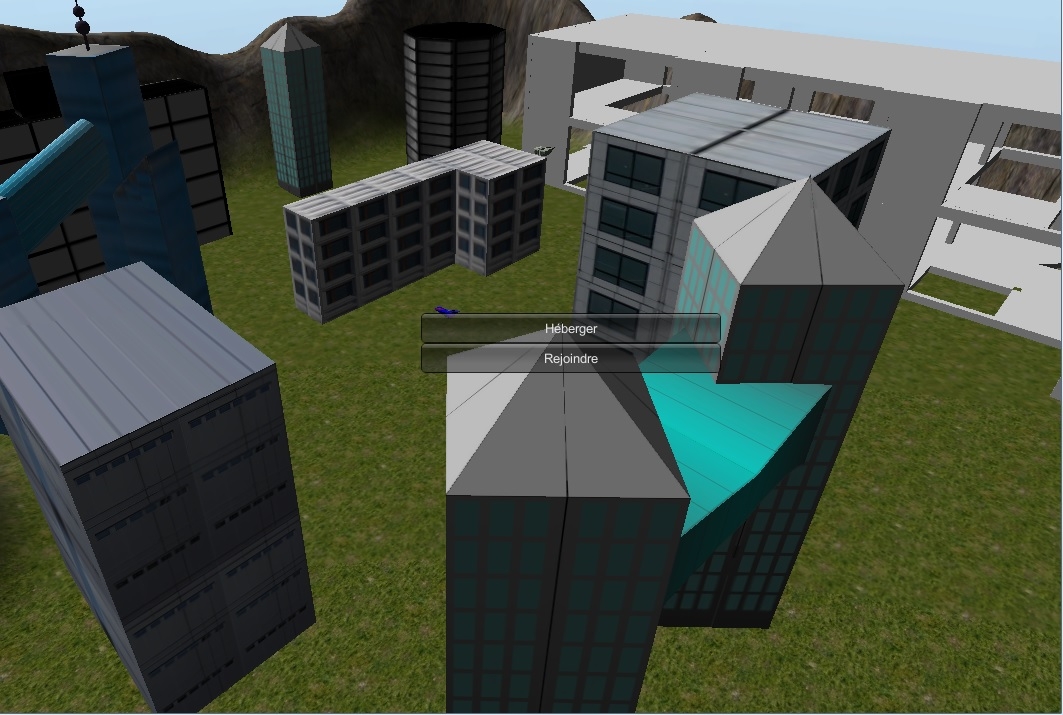
\includegraphics[height=7cm, width=12cm]{lan.jpg}
\end{center}

Les règles du jeu sont les mêmes que dans le mode un joueur ou écran séparé.\\

Le principal problème fut qu'au départ, les joueurs contrôlaient le vaisseau de l'autre joueur et donc devait regarder sur l'autre écran pour jouer. De plus, à trois joueurs, les deux premiers connectés voyaient un seul et même vaisseau qu'il contrôlaient tous les deux pendant que le troisième joueur en pilotait un autre. Le dernier vaisseau quant à lui n'était contrôlé par personne et restait immobile. Au final, ce problème venait de l'assignation des caméras et des scripts aux joueurs lorsqu'ils instanciaient un nouveau vaisseau en arrivant.\\

Au début, nous n'arrivions pas à faire disparaitre le vaisseau d'un joueur lorsqu'il se déconnectait de la partie en ligne. En effet la fonction \textit{Network.Destroy()} ne s'appliquait pas au \textit{prefab} tout entier car il ne contenait pas de \textit{networkView}. Finalement, nous avons intégré cette fonction dans les scripts qui contrôle les déplacements du vaisseau et de la caméra.\\

Lorsque l'on démarre le mode réseau, l'antivirus des ordinateurs peut bloquer le jeu, ou tout au moins demander l'autorisation à l'utilisateur de laisser libre la connexion. Cela n'est pas une très grande gêne car une fois que l'on désactive les pare-feu, tout revient dans l'ordre, mais nous ne savons pas comment la supprimer définitivement. Cela ne nous empêche cependant pas de jouer.\\

\subsection{Quaternions}
Il nous avait été demandé lors de la dernière soutenance de modifier les déplacements des vaisseaux en rajoutant des quaternions pour faire les rotations des vaisseaux. Comme c'était Arthur qui s'était chargé des mouvements à la base, c'est lui qui a modifié le code pour mettre à la place des quaternions. Maintenant, les mouvements sont plus réalistes grâce à l'inertie mais cela rend le jeu un peu plus difficile.\\

Nous n'avions pas utilisé cette technique plus tôt car elle laissait les forces de collisions sur le vaisseau qui le faisaient déplacer après avoir touché un immeuble. En effet le \textit{rigidbody} du vaisseau conservait les collisions subies et donc le rebondissement du vaisseau sur les objets. Dès que le joueur touchait un immeuble, le vaisseau rebondissait et cette force ne s'annulait que très lentement. Nous avons remédié à ce problème en mettant à zéro les déplacements du vaisseau dans la fonction \textit{Update} si le joueur ne bouge pas.\\

Parfois, lorsque le vaisseau tournaient longtemps sur lui-même, il se mettait soudainement à partir dans l'autre sens avant de repartir de la rotation voulue. En effet le quaternion dépassait les 180\textdegree  et donc la rotation s'inversait. En ajoutant un maximum à l'accélération, on a pu régler facilement ce petit imprévu qui rendait le pilotage imprévisible.\\

\subsection{Intelligence artificielle}

Arthur a commencé à faire une intelligence artificielle pour pouvoir jouer contre des vaisseaux contrôlés par l'ordinateur. Pour le début nous voulions faire un algorithme de \textit{pathfiding}. C'est un algorithme qui permet de calculer la trajectoire la plus courte d'un point A à un point B en évitant les obstacles, et donc permet à une intelligence artificielle de se déplacer facilement. Cependant la 3D nous a posé problème, car on ne peut représenter facilement le terrain sous forme de tableau. Il faudrait utiliser un graphe, mais non seulement nous ne savons pas comment le faire, mais en plus il faudrait en faire un différent pour chaque carte, et nous n'avons pas eu le temps.\\

Nous avons donc opté pour une autre technique : devant le vaisseau, nous avons rajouté des cylindres invisibles qui détectent des collisions avec les murs. Lorsque cela se produit, le vaisseau ralentit puis tourne en conséquence pour ne pas rentrer dans l'obstacle. Il y a quatre cylindre : un pour la gauche, un pour la droite, un pour le haut et un pour le bas. Ils sont placés de manière conique pour mieux détecter les immeubles. Le vaisseau circule donc entre les bâtiments qu'il détecte et évite.

\begin{center}
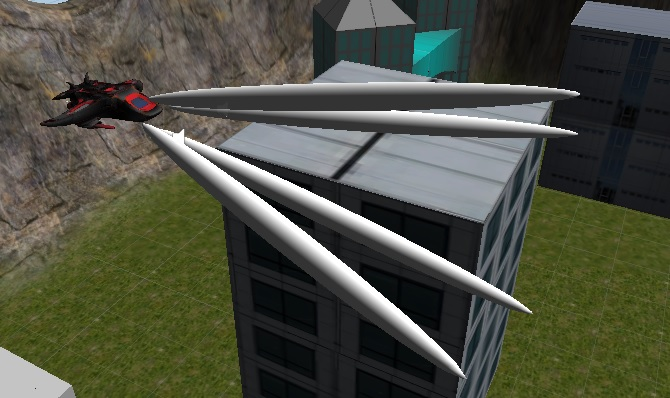
\includegraphics[height=7cm, width=12cm]{ia.jpg}
\end{center}

Nous avons remarqué que cela ne fonctionnait pas pour les objets qui avait pour \textit{collider} un\textit{ Mesh Collider}. Nous avons donc rajouté des \textit{Box Collider} à tous les bâtiments pour qu'il ne fonce pas dedans, tout en veillant à ce qu'il ne crée pas de collision avec les autres vaisseaux. Cependant le vaisseau continue parfois de vouloir passer au travers du terrain ou des limites invisibles du niveau, car les \textit{collider} sont différents.\\

Cette intelligence artificielle n'est pas encore optimale : elle se prend toujours des terrains ou murs invisibles, et surtout elle ne cherche pas le joueur adverse pour le battre. Elle se contente de tirer en continue droit devant elle pendant qu'elle se déplace en slalomant entre les immeubles.\\

\subsection{Menus}

Le menu a été complété par Arthur. Il a rajouté la sélection de la qualité d'image dans le menu option pour pouvoir choisir en fonction de la performance de son ordinateur les meilleurs graphismes possibles.\\

\begin{center}
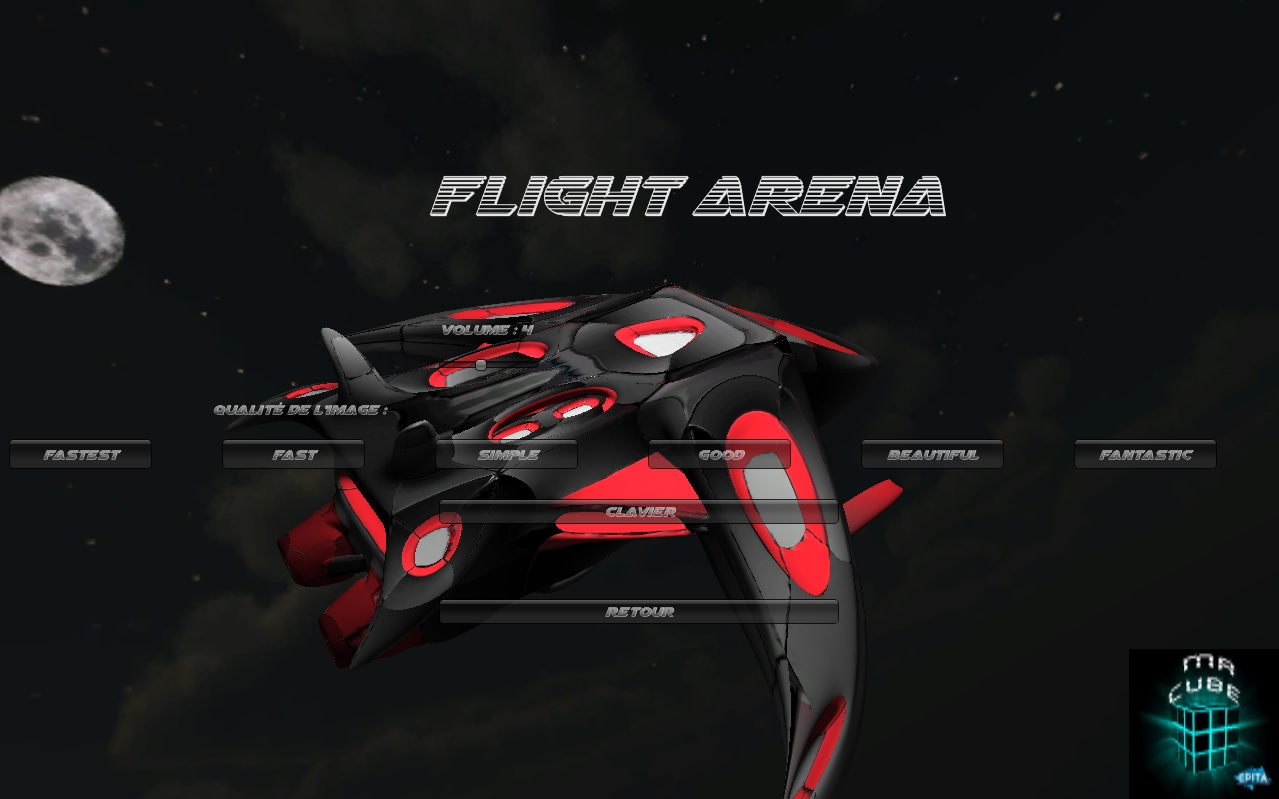
\includegraphics[height=7cm, width=12cm]{menu_option.jpg}
\end{center}

Il a aussi fait en sorte que le joueur puisse choisir le vaisseau qu'il veut piloter parmi les différents proposés avant de commencer la partie parmi les trois proposés faits par Vincent. Ce n'est qu'une différence d'habillage, les trois vaisseaux ont les mêmes propriétés physiques (vitesse, rotation \dots )\\

\begin{center}
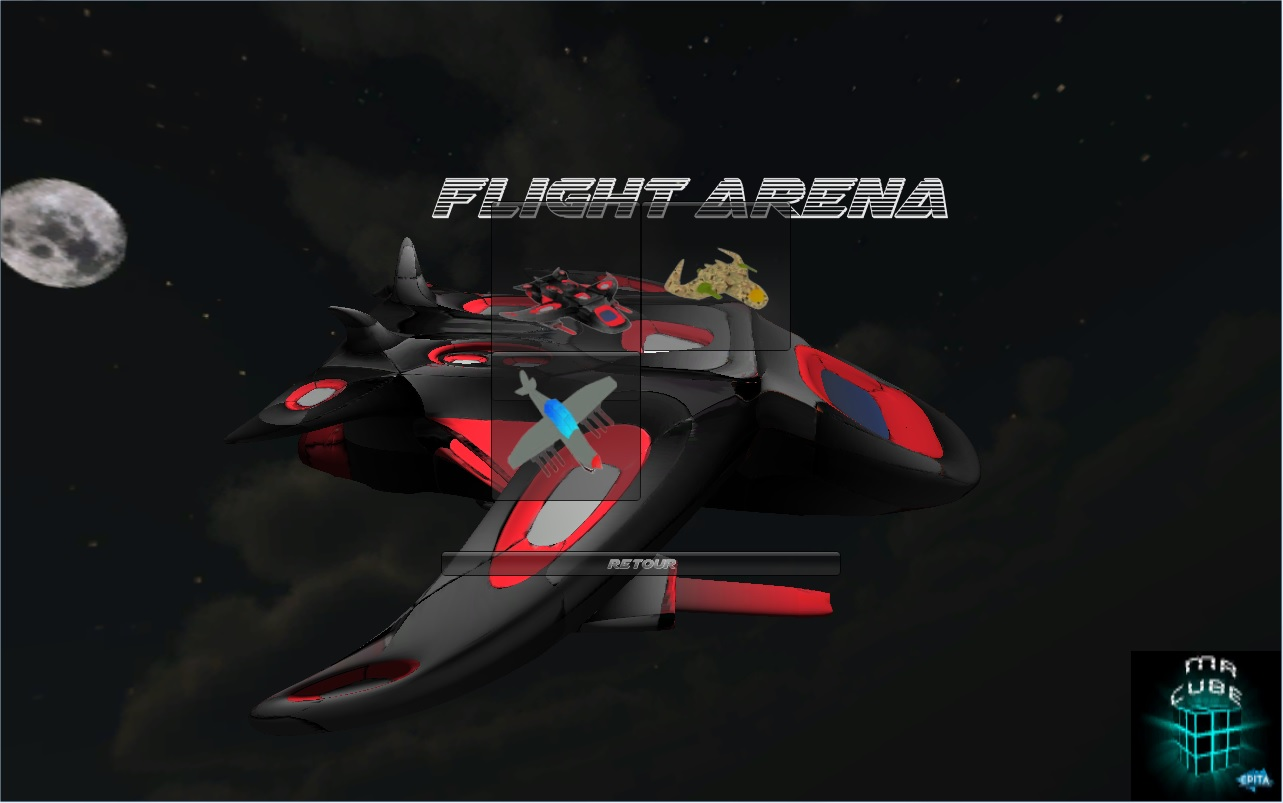
\includegraphics[height=7cm, width=12cm]{menu_selection.jpg}
\end{center}

Pour pouvoir changer de vaisseau au démarrage d'une scène, il a fallu mettre les trois vaisseaux dans des \textit{prefab} que l'on instancie juste à l'arrivée dans la scène. Cependant, nous avons remarqué que lors de l'exportation des modèles depuis Blender vers Unity, la rotation de l'objet était modifiée ce qui faisait que l'on voyait le dessous du vaisseau 2 et le côté du vaisseau 3. Nous avons alors recherché sur internet pour voir que lors de l'exportation en format \textit{fbx}, il fallait choisir les axes pour définir l'avant et le haut de l'objet. Ainsi tout se remettait à l'endroit et le vaisseau était vu correctement.

Pour pouvoir définir quel vaisseau devait être instancié au démarrage, nous avons utilisé un entier stocké dans un \textit{PlayerPrefs} qui est défini dans la scène du menu puis récupéré dans les scènes de jeu.\\

Au départ, nous voulions faire en sorte que le joueur puisse choisir la répartition des touches de son clavier s'il voulait changer ses commandes pour être plus à l'aise. Cependant, nous ignorons totalement comment le faire et Arthur n'a rien trouvé sur internet pour le faire, même dans la documentation de Unity. Nous avons donc abandonné cette idée, comme nous l'avons dit dans la partie de retard.\\

Il a aussi été rajouté le texte "Chargement..." lors du chargement d'une partie, pour que le joueur comprenne qu'il doit attendre, alors qu'avant il n'y avait aucune indication. Ce n'est qu'un détail mais il a son importance.\\

\subsection{Ce qu'Arthur doit faire pour la soutenance finale}
Pour la dernière soutenance, Arthur va surtout s'occuper de compléter et de terminer l'intelligence artificielle. Elle doit pouvoir rechercher un minimum l'adversaire, voire même esquiver les attaques. Le but est qu'elle soit le plus générique pour ne pas avoir besoin de la modifier pour chaque nouvelle carte. Nous ne voulons pas créer de points sur la carte tel que l'intelligence artificielle se déplace de l'un à l'autre. Si le temps le permet, il pourra éventuellement faire plusieurs "attitudes" aux vaisseaux gérés par l'ordinateur : plus agressif, plus prudent \dots  etc. Cela les rendrait moins prévisible et plus réaliste, dans le sens plus humain.\\

Si des modifications doivent être apportées au script ou surtout au multijoueur, c'est lui qui s'en chargera, ou au moins qui aidera vu que c'est lui qui s'en ait chargé pour l'instant. Cela peut être l'ajout de vaisseaux dans les menus et au démarrage des scènes, des ajouts de missiles \dots etc.\\

En cas de retard, il pourra aider dans l'élaboration des cartes, pour placer les bâtiments et faire un peu de gameplay.

\chapter{Pour la prochaine soutenance}
Pour la dernière soutenance, le projet devra être fini.\\

 Nous allons nous concentrer sur l'intelligence artificielle qui est en retard pour qu'elle soit le plus opérationnelle possible. Elle ne se contentera plus de se déplacer aléatoirement parmi les immeubles, mais attaquera les ennemis et essayera de survivre sous les tirs ennemis. On pourra aussi en rajouter dans les autres modes de jeu, nous voulons parler ici du multijoueur en LAN et en écran séparé.\\

Il y aura aussi du contenu supplémentaire, notamment des cartes avec de nouveaux bâtiments qui pourront ajouter du gameplay comme des éoliennes ou d'autres sortent de bâtiments mouvants qui obligent les joueurs à slalomer encore plus. Il pourra y avoir aussi des vaisseaux non-joueurs, qui sont juste d'autres obstacles mobiles, comme des citoyens innocents subissant la bataille.\\

Le menu sera adapté en conséquence pour que le joueur choisisse sa carte avant de jouer, sans doute assez similaire au système de choix de vaisseau qui existe actuellement. On pourra aussi choisir le nombre de vaisseaux contrôlés par l'ordinateur pendant la partie.

Nous essayerons de rajouter par des moyens détournés de rajouter le choix des touches pour jouer dans le menu des options, mais cela reste optionnel.\\

Toutes les nouveautés seront jouables en multijoueur, que ce soit sur le mode écran séparé ou le mode réseau LAN. Nous essayeront aussi de rajouté le contrôle à la manette, pour les joueurs qui se sentent plus à l'aise avec pour jouer que sur clavier, et surtout pour éviter de se gêner en écran partagé.\\

Tout le contenu sera disponible en téléchargement sur le site internet, en ligne. Celui-ci sera achevé, avec le projet disponible dans son intégralité. On pourra suivre l'évolution du jeu au fur et à mesure avec le contenu ajouté, et des renseignement sur tout ce qui tourne autour : les développeurs, les partenaires \dots \\

Le jeu sera fournit avec une installation sur CD-ROM, avec une boite prévue à cette effet. \\ \\ \\ \\ \\ \\

\begin{center}
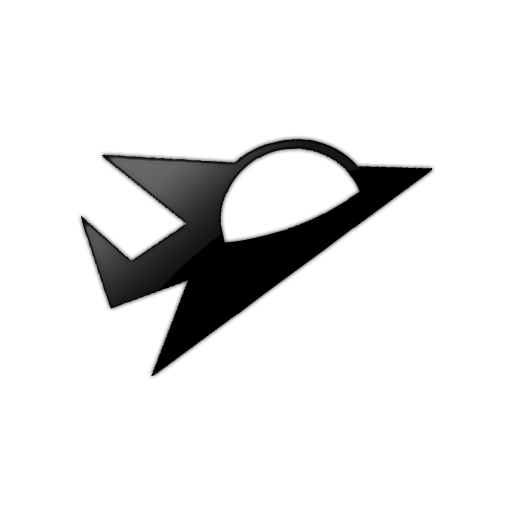
\includegraphics[height=4cm, width=4cm]{vaisseux_petit.png}
\end{center}

\end{document}